%!TEX root = ../2019_7_Ozgumus_Semsi_Yigit.tex

\begingroup

This chapter presents the modifications applied to aforementioned approaches to improve the performance 
of the anomaly detection. All the discussed models measures its performance metric on well known datasets, 
such as CIFAR-10 \cite{cifar10} and SVHN \cite{Netzer2011ReadingDI}. The dataset used in this thesis presents 
additional challenges to this problem we aim to solve. The first section will introduce its dataset to the 
reader and will give examples. Next section will discuss the shortcomings of the previous approaches regarding 
the interpretation of the dataset and detection of the existent anomalies. Sections \ref{sec:encebgan} and 
\ref{sec:sencebgan} will explain the modified architecture and the significance of the changes.

\section{SEM Image Dataset}
\label{sec:sem}

Nanofibrous materials acquired increasingly significant demand from variety of fields in the Industry. 
It constitutes a foundation material for a lot of products including areas in medicine, filtration, sensors 
and manufacturing applications. \cite{carrera2016defect}. Despite the demand and continuous research 
development towards its production, manufacturing nanofibrous materials is still  challenge for scaled of 
mass production. Several techniques for producing nanofibers have been presented in the literature. 
\cite{carrera2016defect}. Electrospinning method is the focus of this anomaly detection task. It produces 
a structure which consists of filaments woven in with randomized geometric pattern. You can see one of the images 
of the material produced without any anomalies in figure \ref{fig:data_norm}.

\begin{figure}[h!]
	\centering
	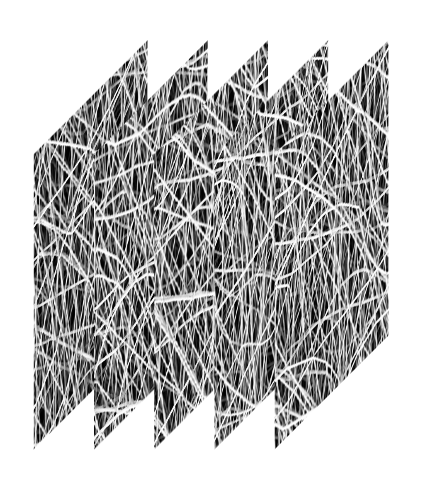
\includegraphics[width=0.75\textwidth]{dataset}
	\caption{Part of Training Dataset from the SEM Image Dataset \cite{sem}}
	\label{fig:data_norm}
\end{figure}

Dataset consists of 5 images with no anomalies and 40 sample images that have various types of anomalous regions. To preserve 
computational efficiency without sacrifising from performance, training dataset and testing dataset is sampled from SEM image dataset.
\begin{figure}[h!]
	 \subfloat[Normal regions]{
		\begin{minipage}[c][0.8\width]{0.5\textwidth}
			\centering
			\fbox{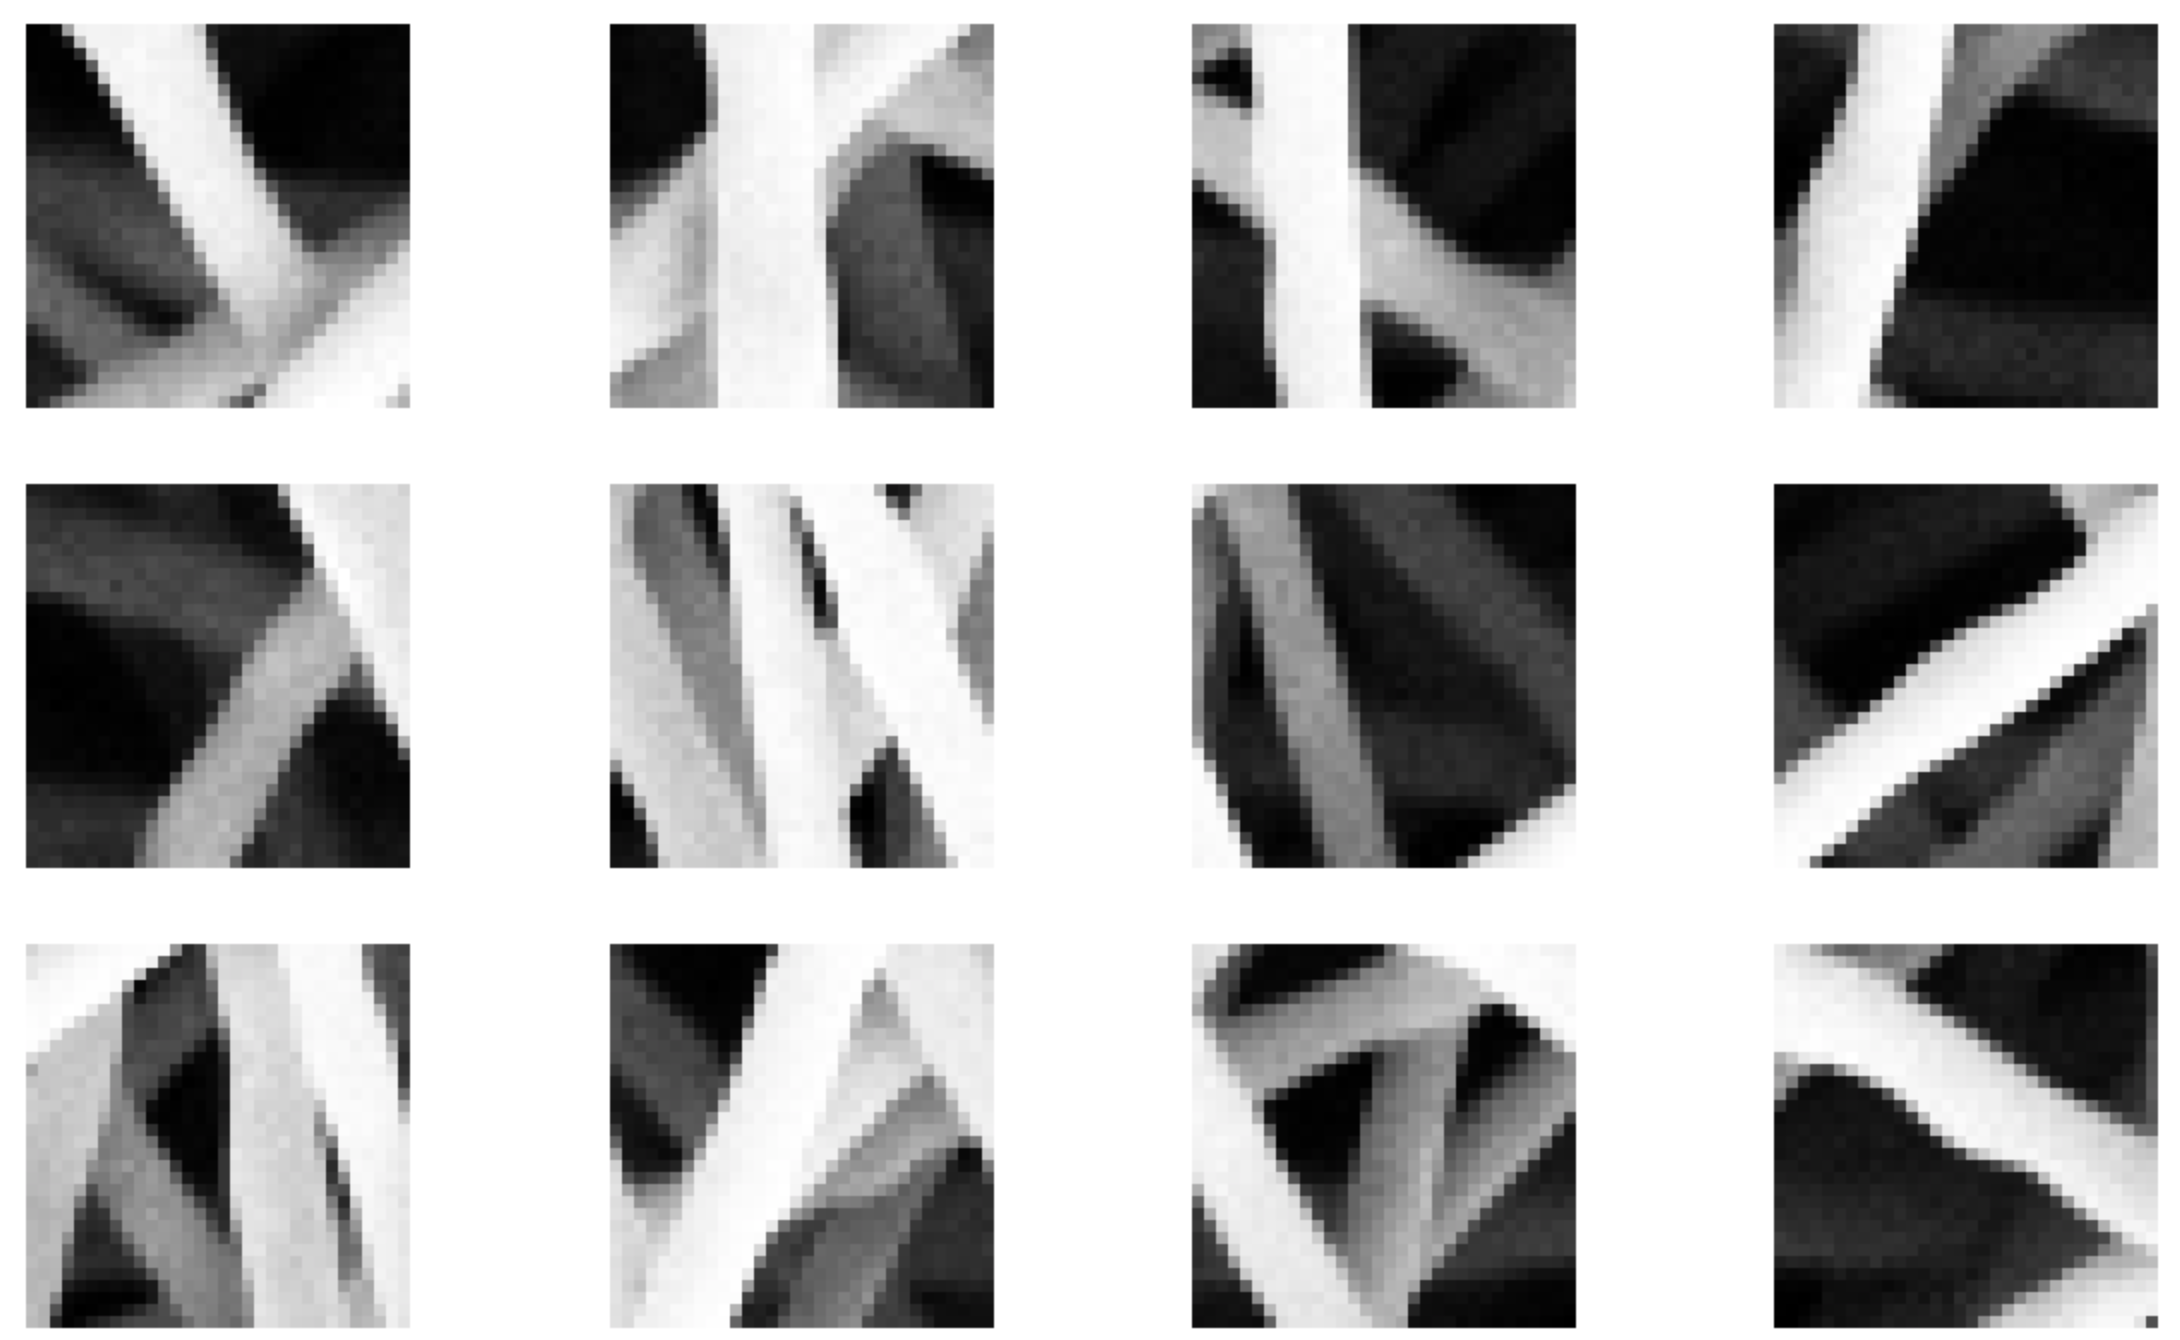
\includegraphics[width=1\textwidth]{sample_normal}}
			\label{fig:data_sample_normal}
	\end{minipage}}
	\hspace*{\fill}%
	\subfloat[Anomalous regions]{
		\begin{minipage}[c][0.8\width]{0.5\textwidth}
			\centering
			\fbox{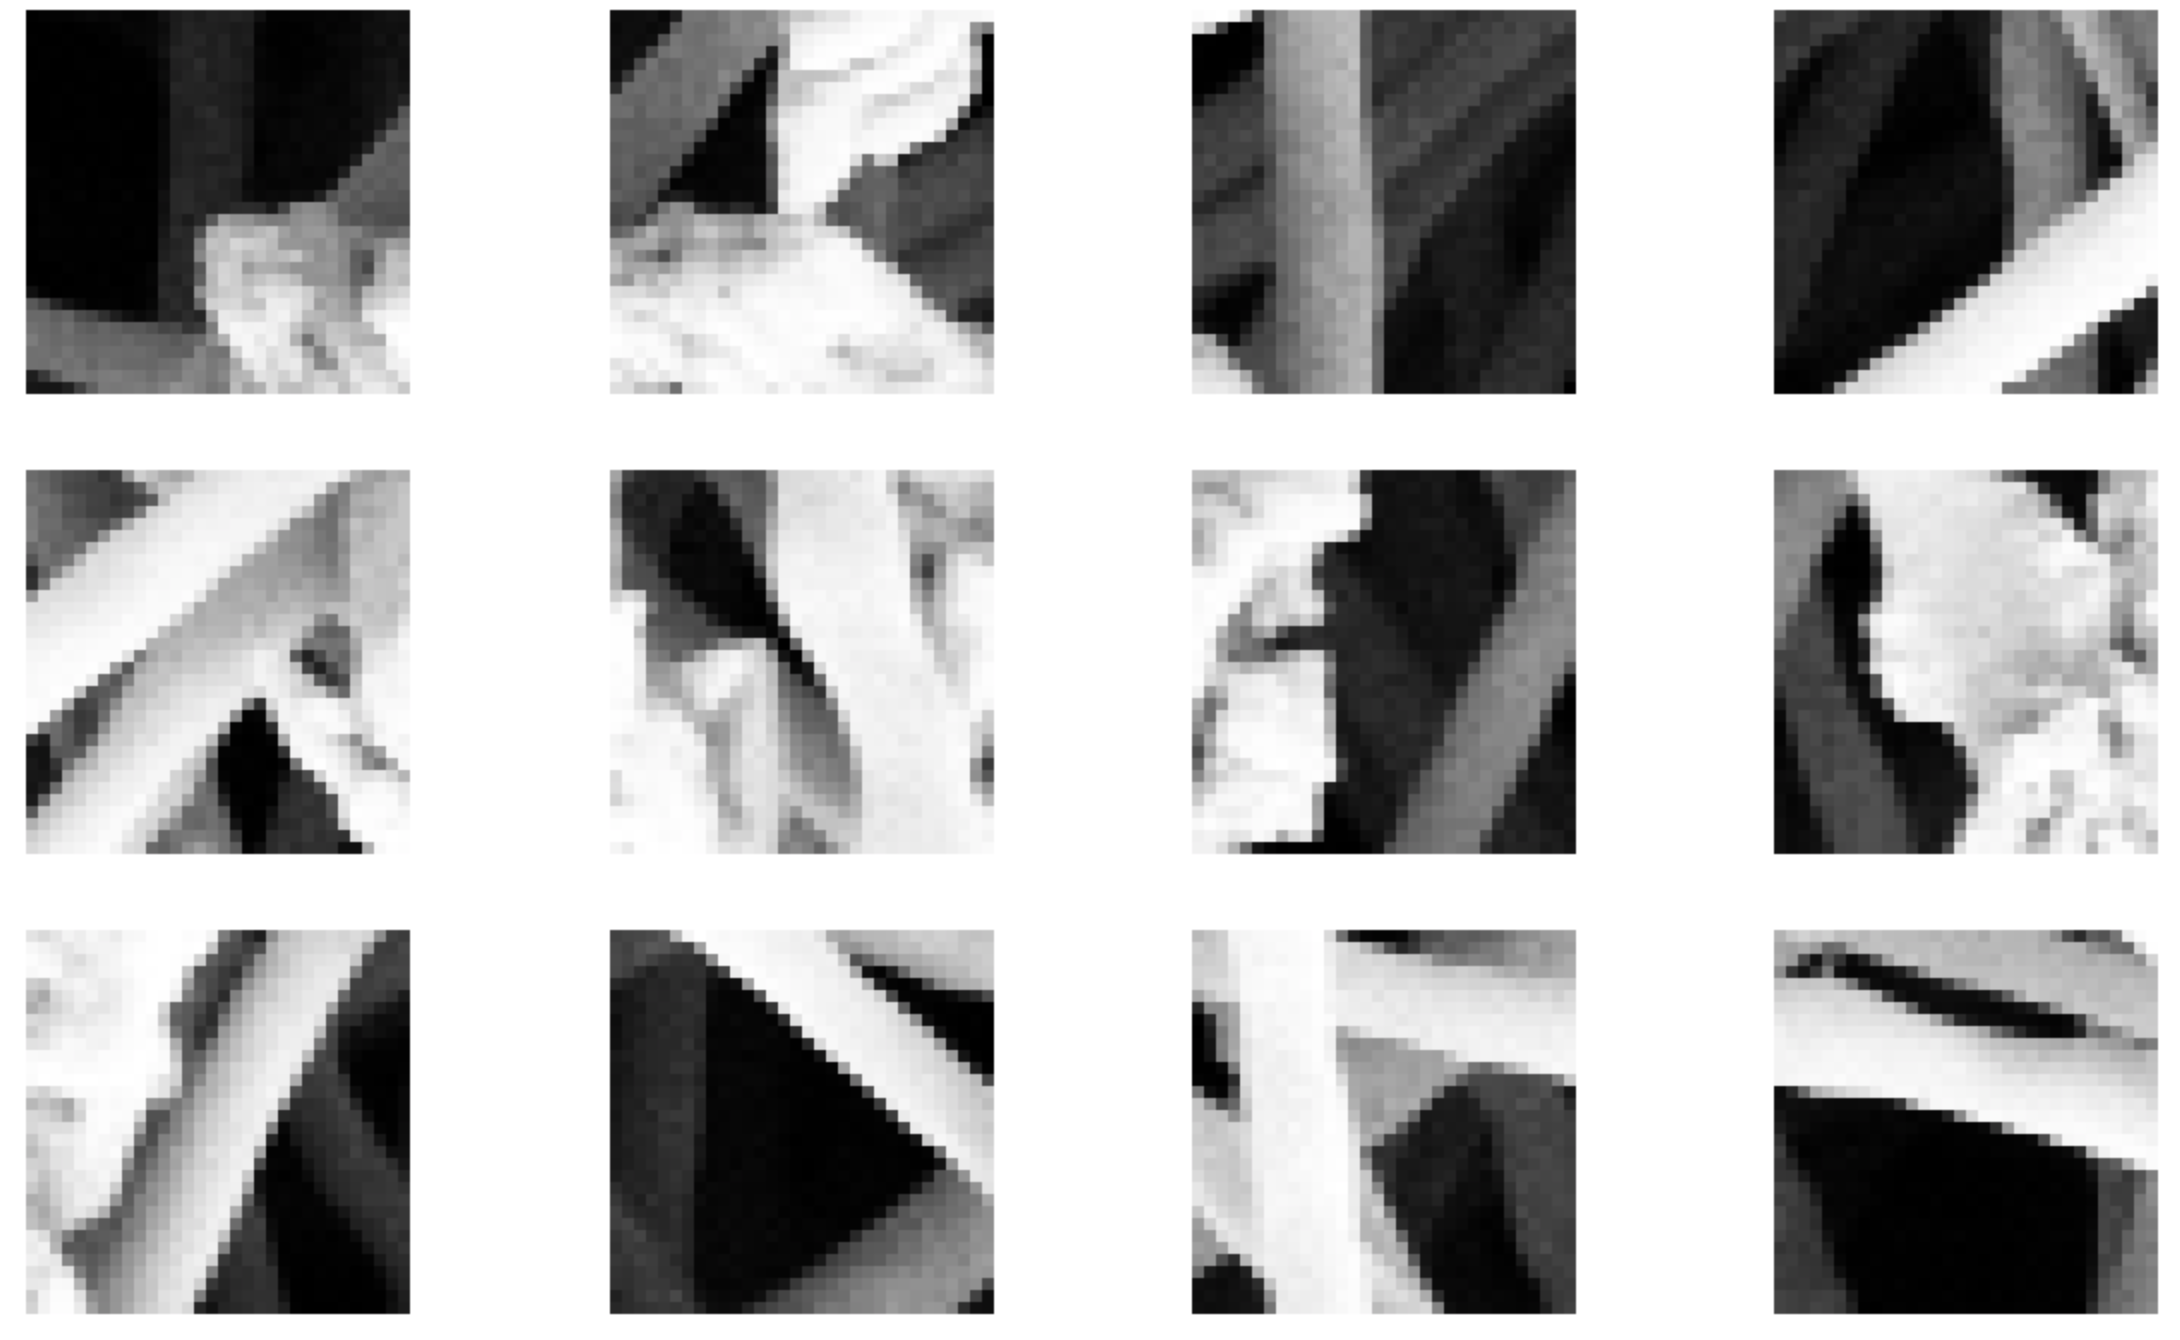
\includegraphics[width=1\textwidth]{sample_anomaly}}
			\label{fig:data_sample_anomaly}
	\end{minipage}}
	\caption{Normal and Anomalous region patches for the training and testing}
	\label{fig:data_samples}
\end{figure}

$32 \times 32$ patches are selected as the image size as if proposed framework prove useful for the anomaly detection, 
testing the model with other known datasets such as CIFAR10 \cite{cifar10} and SVHN \cite{Netzer2011ReadingDI} would be more convenient. 
$28 \times 28$ patch size is also considered but choosing $28 \times 28$ image size forced model to have less transposed convolution 
layers (see chapter \ref{chap:imp_details} for model details) and GAN models designed with that architecture experienced model collapse 
frequently in the preliminary experiments.
Figure \ref{fig:data_sample_normal} shows the example patches used for the 
training phase. Training dataset consists of patches which contains no anomalies. Figure \ref{fig:data_sample_anomaly} 
shows the anomalous samples which are used in the inference stage. The Anomalous regions can reside in both the topmost layer
or can be hidden in deep in the woven structure.

\section{Analysis of Aforementioned Approaches}
\label{sec:analysis_before}

This section presents an analysis on the performance of GAN based state of the art anomaly detection methods 
presented in section \ref{sec:gan_based_sota} and a discussion to identify the shortcomings of these methods. 
Stabilization issues in the adversarial training stage, the method to calculate the anomaly score, and reconstruction 
issues related to the encoding of latent representation will be discussed.

Proposed methods in chapter \ref{chap:sota} can be further divided into 2 seperate categories with respect to their generator structure. 
\begin{itemize}
	\item Pure GAN ( AnoGAN (\ref{sec:anogan}), BiGAN (\ref{sec:bigan}) and ALAD (\ref{sec:alad}))
	\item Autoencoder Variants (GANomaly and Skip-GANomaly (\ref{sec:ganomaly}))
\end{itemize}

First group has a generator that accepts the noise as an input and uses adversarial training to match the generated sample distribution 
to the input data distribution. The latter uses an autoencoder based decoder behalf of the generator but still employs adversarial training
to learn the latent representation. During the analysis of the first two observations, autoencoder variants will not be considered for discussion 
since their generator network does not suffer from the stabilization issues of GANs.

\subsection{Stabilization of Adversarial Training}

Stabilization of loss functions of generator and discriminator is still an important issue in GAN training. Various appraches and modifications 
are experimented to further improve the training of the GANs and prevent non convergent scenerios.
\cite{methods} and \cite{fm} proposed additional stabilization "tricks" to improve the convergence properties of the objective function 
and prevent mode collapse. These include adding noise with a decay over time to both input image and generated 
sample before putting through discriminator to add a factor of robustness to the discriminator, using soft labels to define the true 
and fake member class instead of the binary truth values and flipping labels of the true and generated images to fool the discriminator even more
and provide higher gradient flow to generator early on in the training to help it learn to generate images better \cite{fm}.

In the training phase of an generative adversarial network, loss values of generator does not portray a traditional convergence line in plots.
Adversarial minimax game prevents the losses of the player networks to converge to a certain limit. If the loss is reaching zero in any case, it indicates 
a problem in the learning capacity of one of the networks. If discriminator loss converges to zero too quickly, it means that it learned to 
discriminate between the real images and the ones generated by the generator network. On the other hand if the generator loss converges to zero 
early in the training  it indicates a mode collapse but situation may arise in even normal looking training sessions. The problem is at some point in the training generator generates an image that perfectly fools the discriminator. If gradients obtained from this loss computation is high enough, generator might stop learning from the gradient flow of discriminator 
and start to generate the same sample in each iteration. This sample also may not be visually similar to the target distribution. This eliminates the 
purpose of having a generator network.

To mitigate these shortcomings, ablation study is performed on all Pure GAN models which consists of previously mentioned training 
improvements with same model capacity and training hyperparameters to create an equal environment for the models. Despite models 
proving a certain performance standard on the benchmark datasets (\cite{cifar10,Netzer2011ReadingDI}), they performed poorly on the SEM 
image dataset (\cite{sem}). More importantly, the training of the networks were unstable enough to prevent to obtain a consistent performance 
benchmark. Obtaining a stable GAN for generating reconstructions is fairly important because it is the first step of the anomaly 
detection framework. Figure \ref{fig:arim_training} presents the generator/discriminator learning graphs and their generation samples 
from the final training epoch.

% Figure with bigan alad anogan graphs and reconstructions
\begin{figure}[h!]
\def\tabularxcolumn#1{m{#1}}
\begin{tabularx}{\linewidth}{@{}XXX@{}}
	\begin{tabular}{ccc}
		\subfloat[AnoGAN generator training]{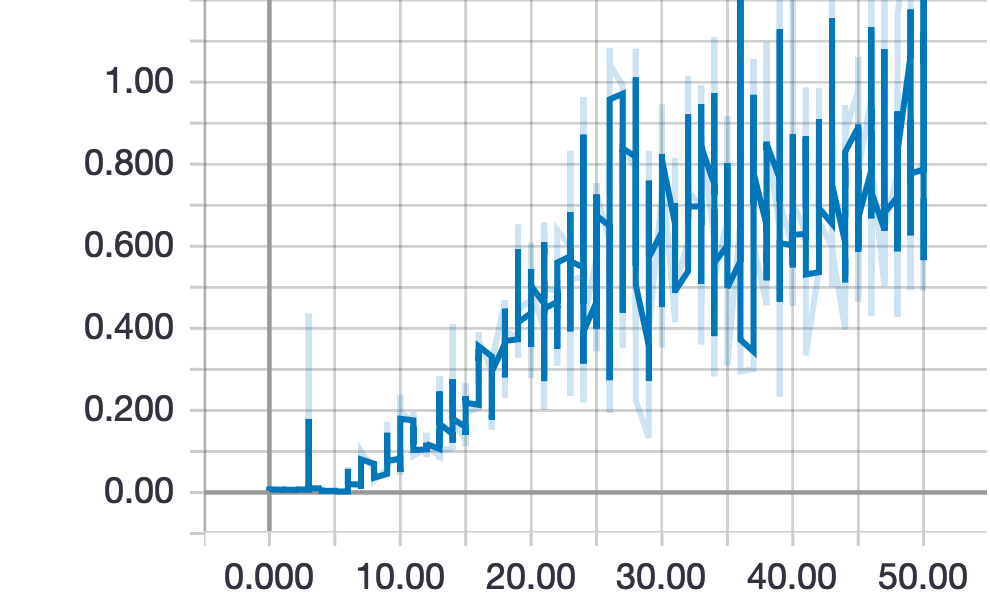
\includegraphics[width=0.3\textwidth]{arim/gan_training/anogan_loss_generator}} 
		& \subfloat[BiGAN generator training]{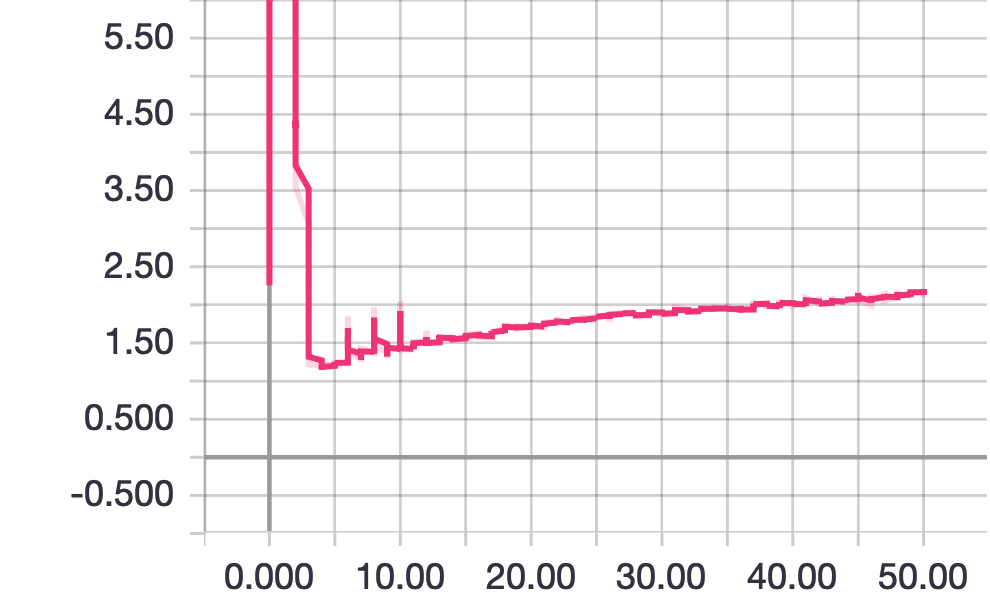
\includegraphics[width=0.3\textwidth]{arim/gan_training/bigan_loss_generator}}
		& \subfloat[ALAD generator training]{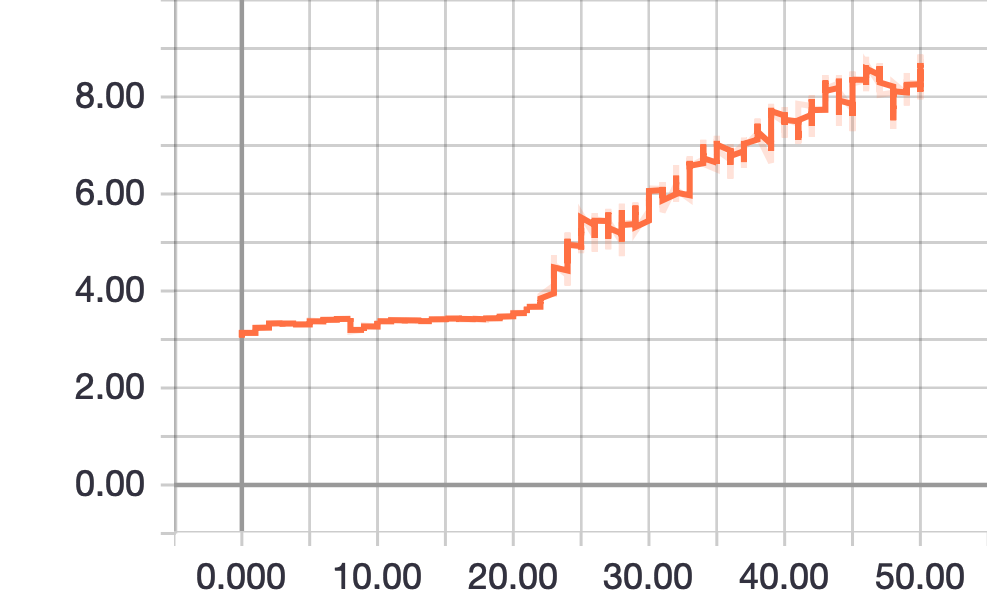
\includegraphics[width=0.3\textwidth]{arim/gan_training/alad_loss_generator}} \\
		\subfloat[AnoGAN discriminator training]{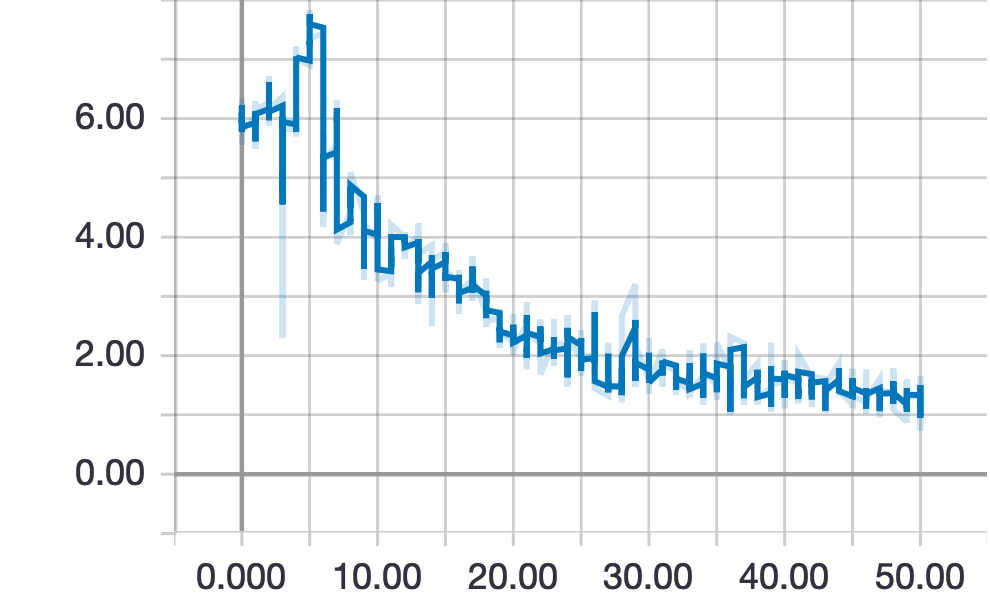
\includegraphics[width=0.3\textwidth]{arim/gan_training/anogan_loss_discriminator}} 
		& \subfloat[BiGAN discriminator training]{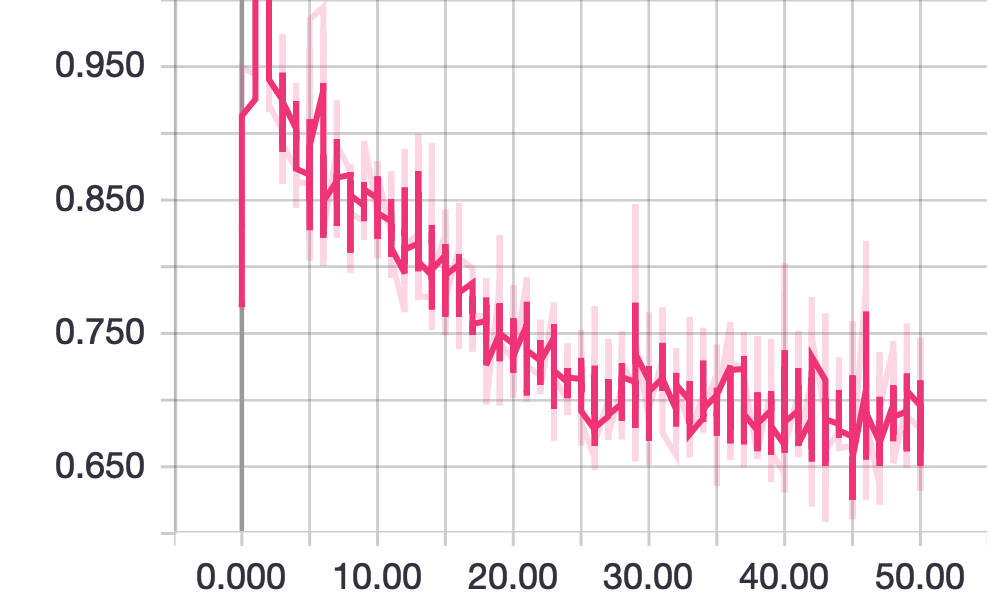
\includegraphics[width=0.3\textwidth]{arim/gan_training/bigan_loss_discriminator}}
		& \subfloat[ALAD discriminator training]{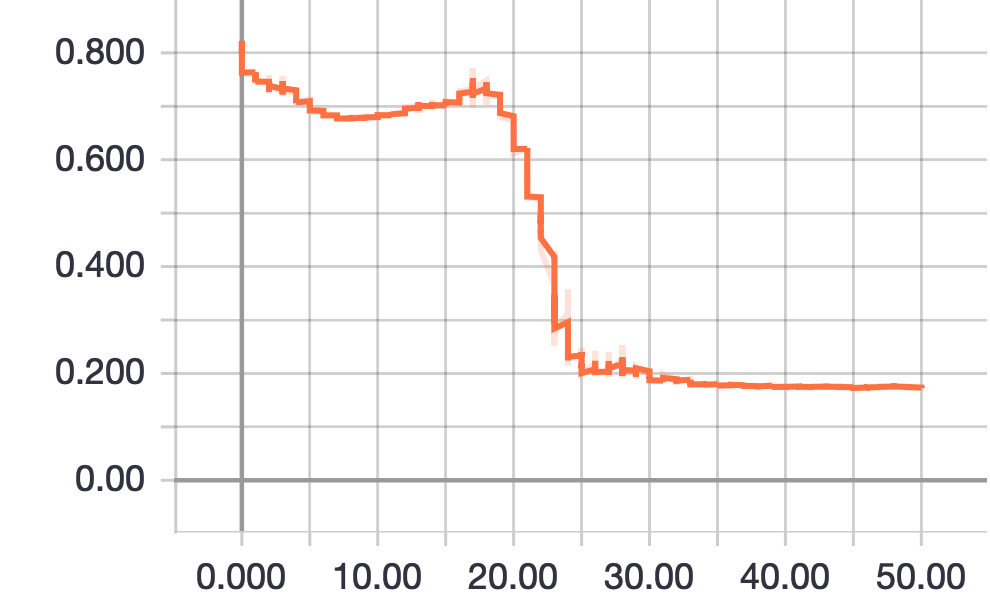
\includegraphics[width=0.3\textwidth]{arim/gan_training/alad_loss_discriminator}} \\
		\subfloat[AnoGAN generated image sample]{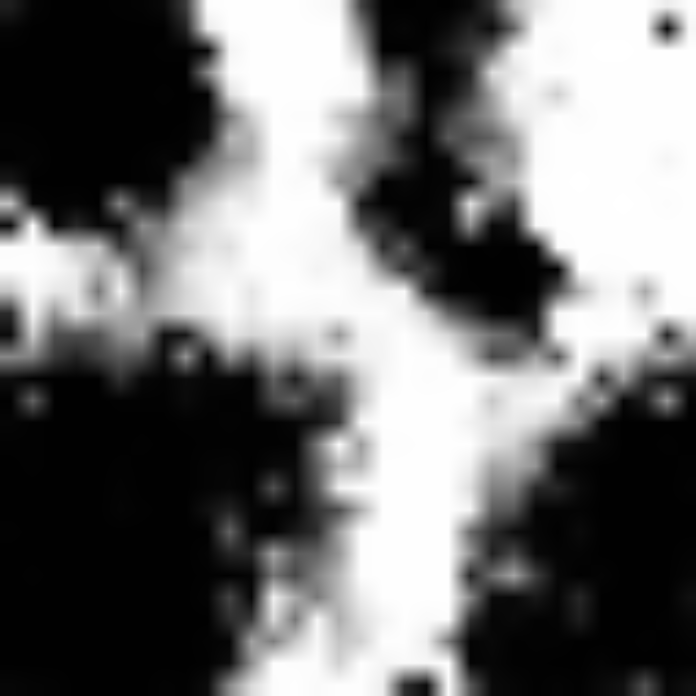
\includegraphics[width=0.3\textwidth]{arim/gan_training/anogan_gan}} 
		& \subfloat[BiGAN generated image sample]{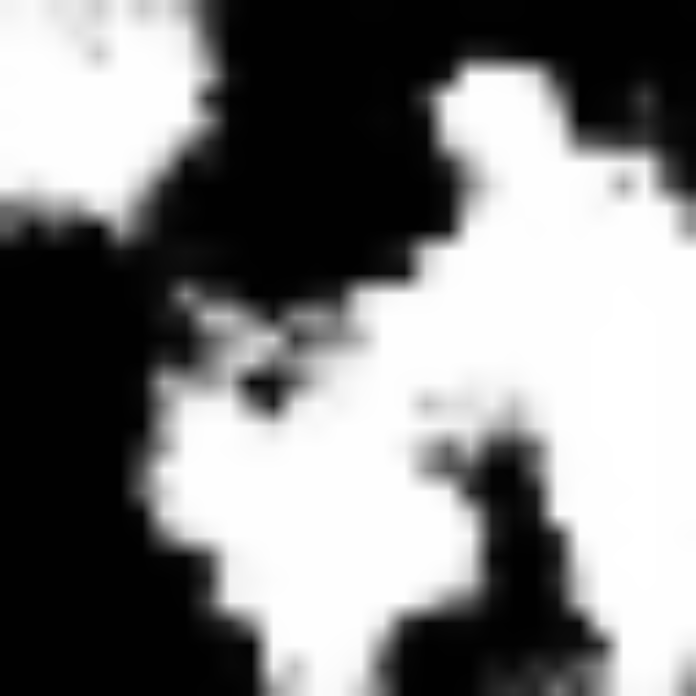
\includegraphics[width=0.3\textwidth]{arim/gan_training/bigan_gan}}
		& \subfloat[ALAD generated image sample]{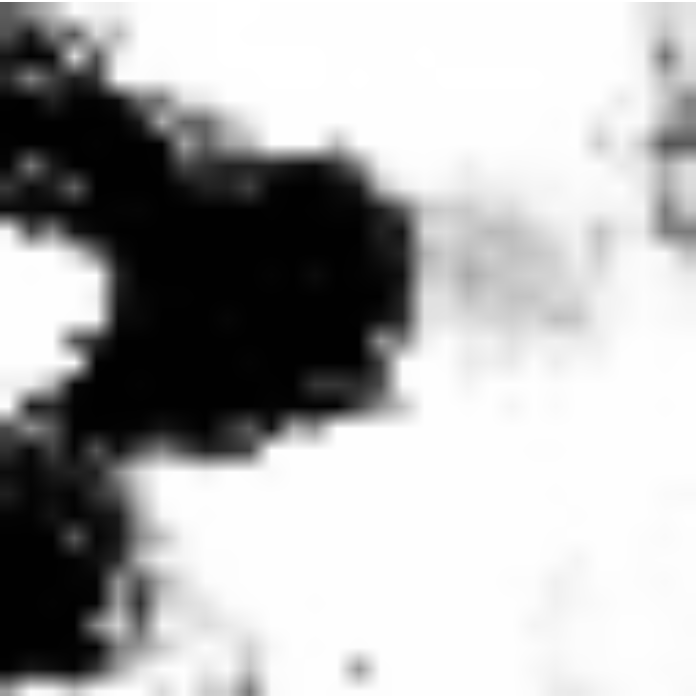
\includegraphics[width=0.3\textwidth]{arim/gan_training/alad_gan}} \\
	\end{tabular}
	\end{tabularx}
	\caption{Training information for the Pure GAN models. For graphs, x axis is the number of epochs and the y axis is the loss value}\label{fig:arim_training}
\end{figure}
%%%
As seen in the figure, discriminator is gradually learning to differentiate between the real and generated image while 
the generator network does not seem to set its loss to a certain level as desired. This trend is observed in the majority of the 
experiments and in the ablation study as well. From the perspective of the image generation, samples generated from GANs are not contextually 
sound enough to represent the target distribution of the SEM image dataset. To obtain a more concise observation the reconstructions of these GANs 
will also be inspected. 

Considering the results of these experiments, training objective of the EBGAN model is adopted to obtain a more stable training with our dataset.  (See eqn. \ref{eqn:ebgan_used})
\begin{equation}
\label{eqn:ebgan_used}
\begin{aligned}
	D(x)&=\|\operatorname{Dec}(E n c(x))-x\|\\[5pt]
	V(G, D) &= D(G(z)) + D(x)+[m-D(G(z))]^{+} \\[5pt]
 	\mathcal{L}_{D}(x, z) &=D(x)+[m-D(G(z))]^{+} \\[5pt]
  	\mathcal{L}_{G}(z) &=D(G(z))
\end{aligned}
\end{equation}

Defining loss function as a value of energy still preserves the adversarial aspect of the objective function. An auto encoder network acts as a 
discriminator module and attains an energies to the real and fake image samples with high energy values assigned to generated images. Generator 
tries to "fool" the discriminator to decrease the amount of energy fake image is assigned. Here the energy term is described as the ability of discriminator to reconsturct the given output, so it is a reconstruction error based value. 

Using energy based GAN proved useful to obtain a consistent performance without having issues with the argued stabilization issues. Details regards to 
its training and model's reconstruction capability will be discussed in its own section.
\subsection{Convergence of Encoder Training}

\begin{figure}[h!]
	\def\tabularxcolumn#1{m{#1}}
	\begin{tabularx}{\linewidth}{@{}XXX@{}}
		\begin{tabular}{ccc}
			\subfloat[BiGAN Encoder Training]{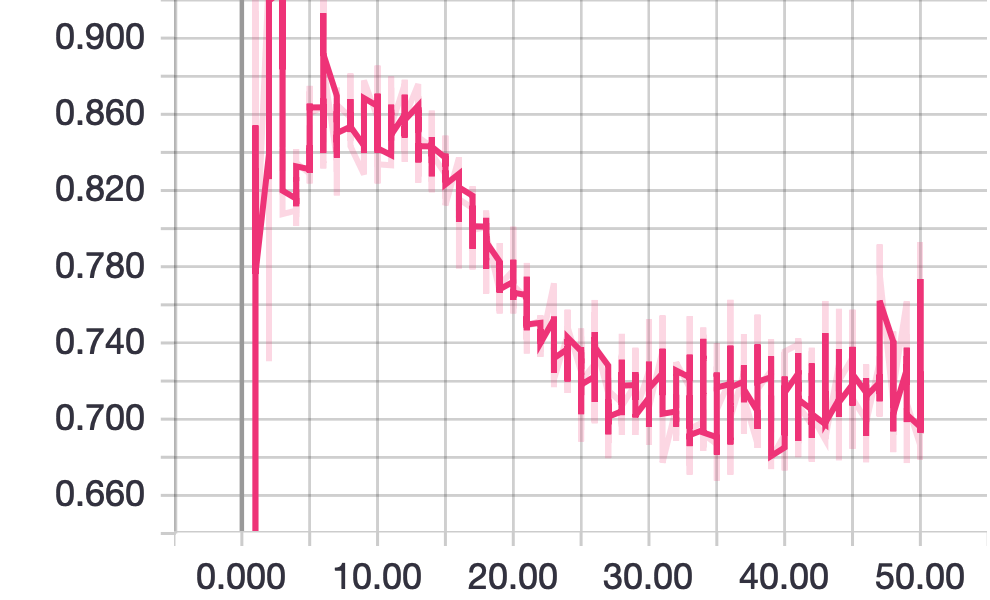
\includegraphics[width=0.3\textwidth]{arim/encoder_conv/bigan_loss_encoder}} 
			& \subfloat[ALAD Encoder Training]{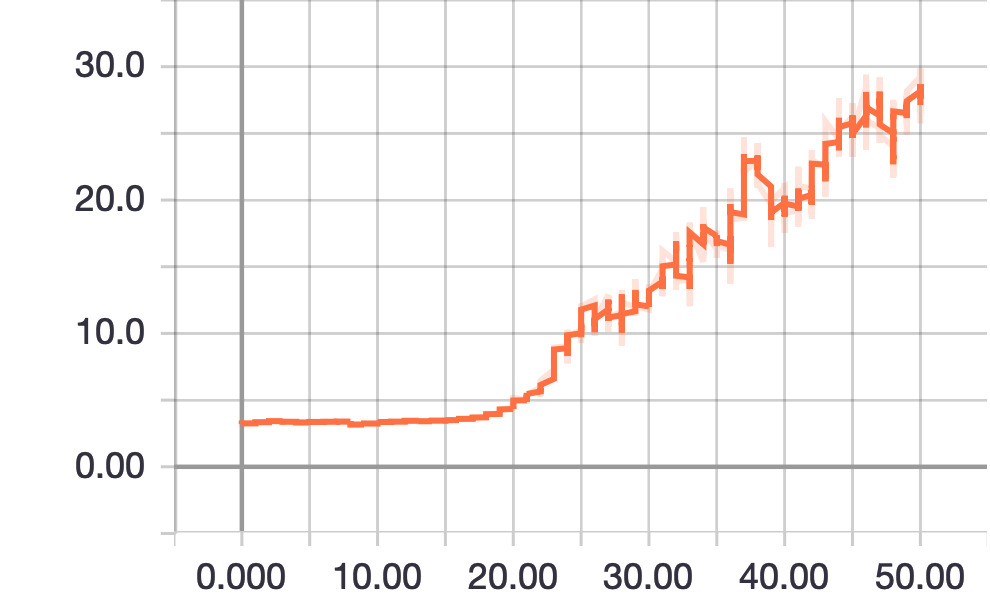
\includegraphics[width=0.3\textwidth]{arim/encoder_conv/alad_loss_encoder}}
			& \subfloat[ENCEBGAN Encoder Training]{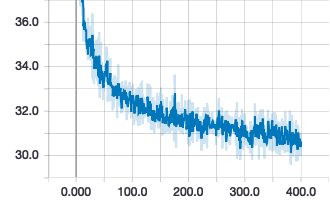
\includegraphics[width=0.3\textwidth]{arim/encoder_conv/enceb_loss_encoder}} \\
		\end{tabular}
	\end{tabularx}
	\caption{}\label{fig:arim_encoder}
\end{figure}
\begin{figure}[h!]\ContinuedFloat	
	\def\tabularxcolumn#1{m{#1}}
	\begin{tabularx}{\linewidth}{@{}XXX@{}}
		\begin{tabular}{ccc}
			\subfloat[AnoGAN Query Image]{
\includegraphics[width=0.3\textwidth]{arim/encoder_conv/anogan_sample}} 
			& \subfloat[BiGAN Query Image]{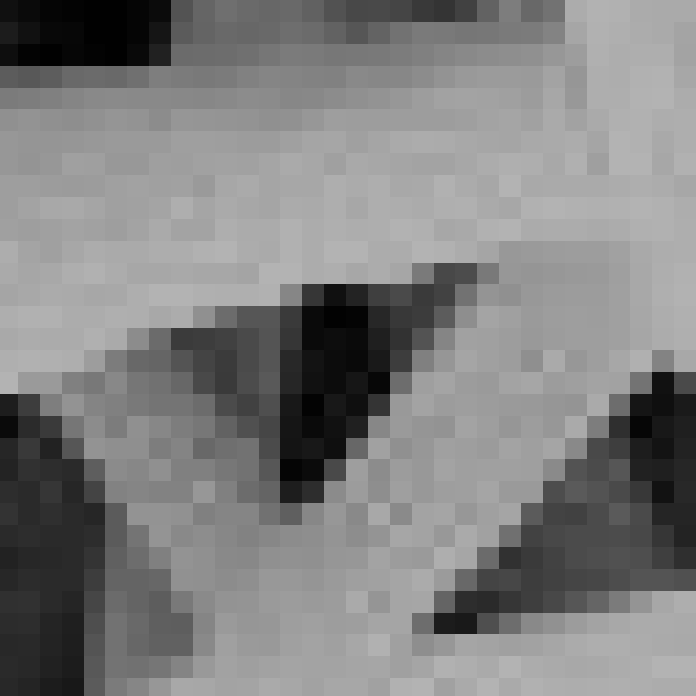
\includegraphics[width=0.3\textwidth]{arim/encoder_conv/bigan_sample}}
			& \subfloat[ALAD Query Image]{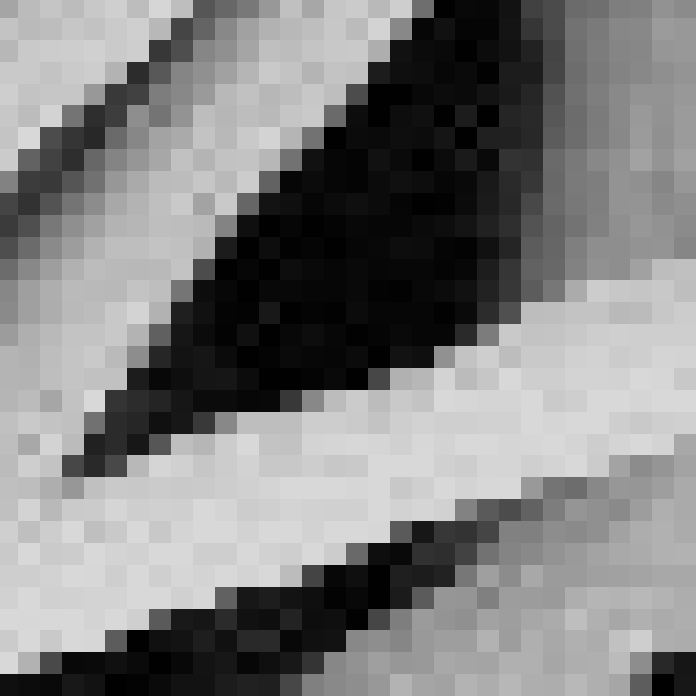
\includegraphics[width=0.3\textwidth]{arim/encoder_conv/alad_sample}} \\
			\subfloat[AnoGAN Reconstruction]{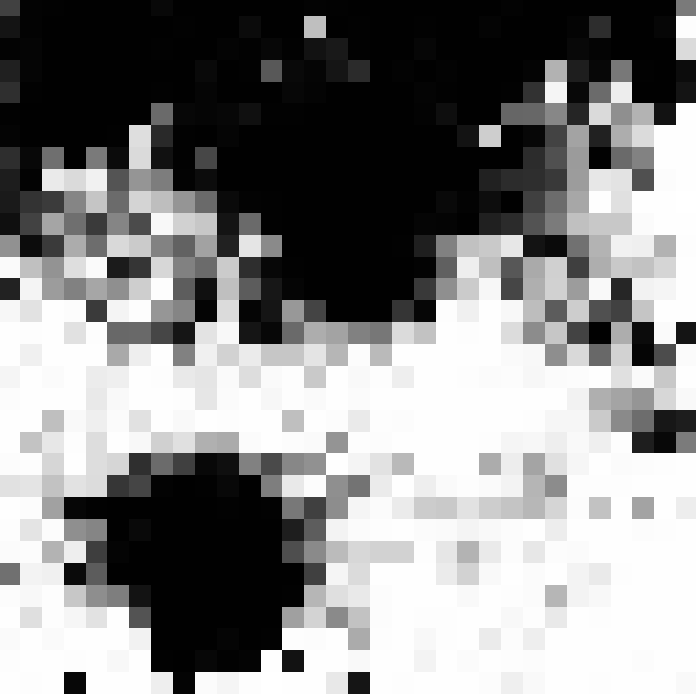
\includegraphics[width=0.3\textwidth]{arim/encoder_conv/anogan_reconstruct}} 
			& \subfloat[BiGAN Reconstruction]{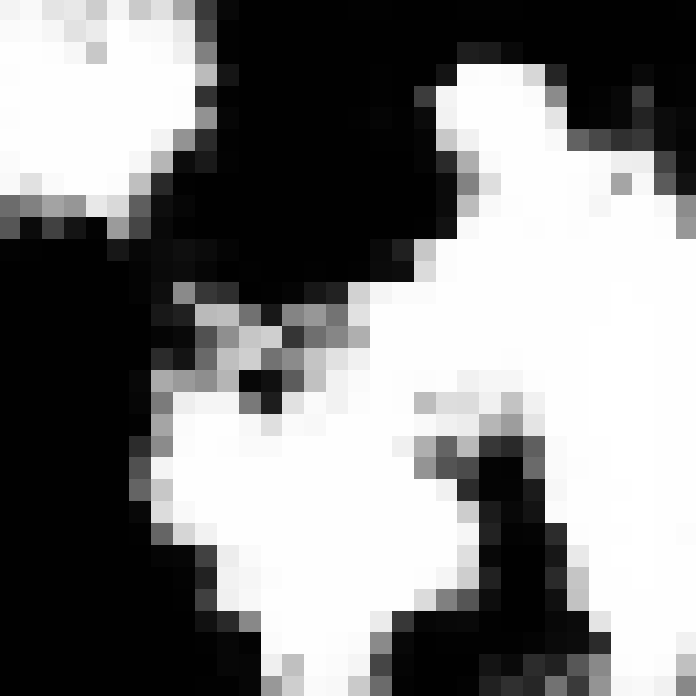
\includegraphics[width=0.3\textwidth]{arim/encoder_conv/bigan_reconstruct}}
			& \subfloat[ALAD Reconstruction]{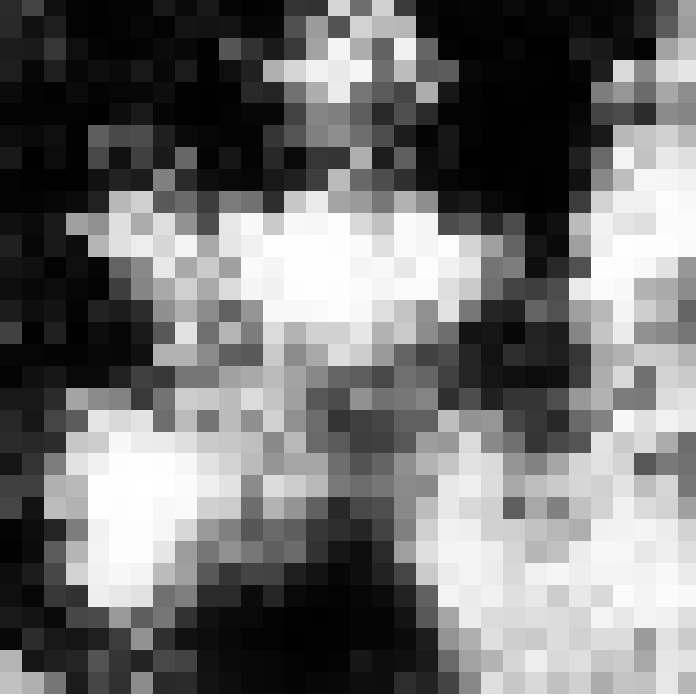
\includegraphics[width=0.3\textwidth]{arim/encoder_conv/alad_reconstruct}} \\
		\end{tabular}
	\end{tabularx}
	\caption{}\label{fig:arim_encoder}
\end{figure}

\subsection{Encoded Energy Based Generative Adversarial Network}
\label{sec:encebgan}

\begin{figure}[h!]
	\centering
	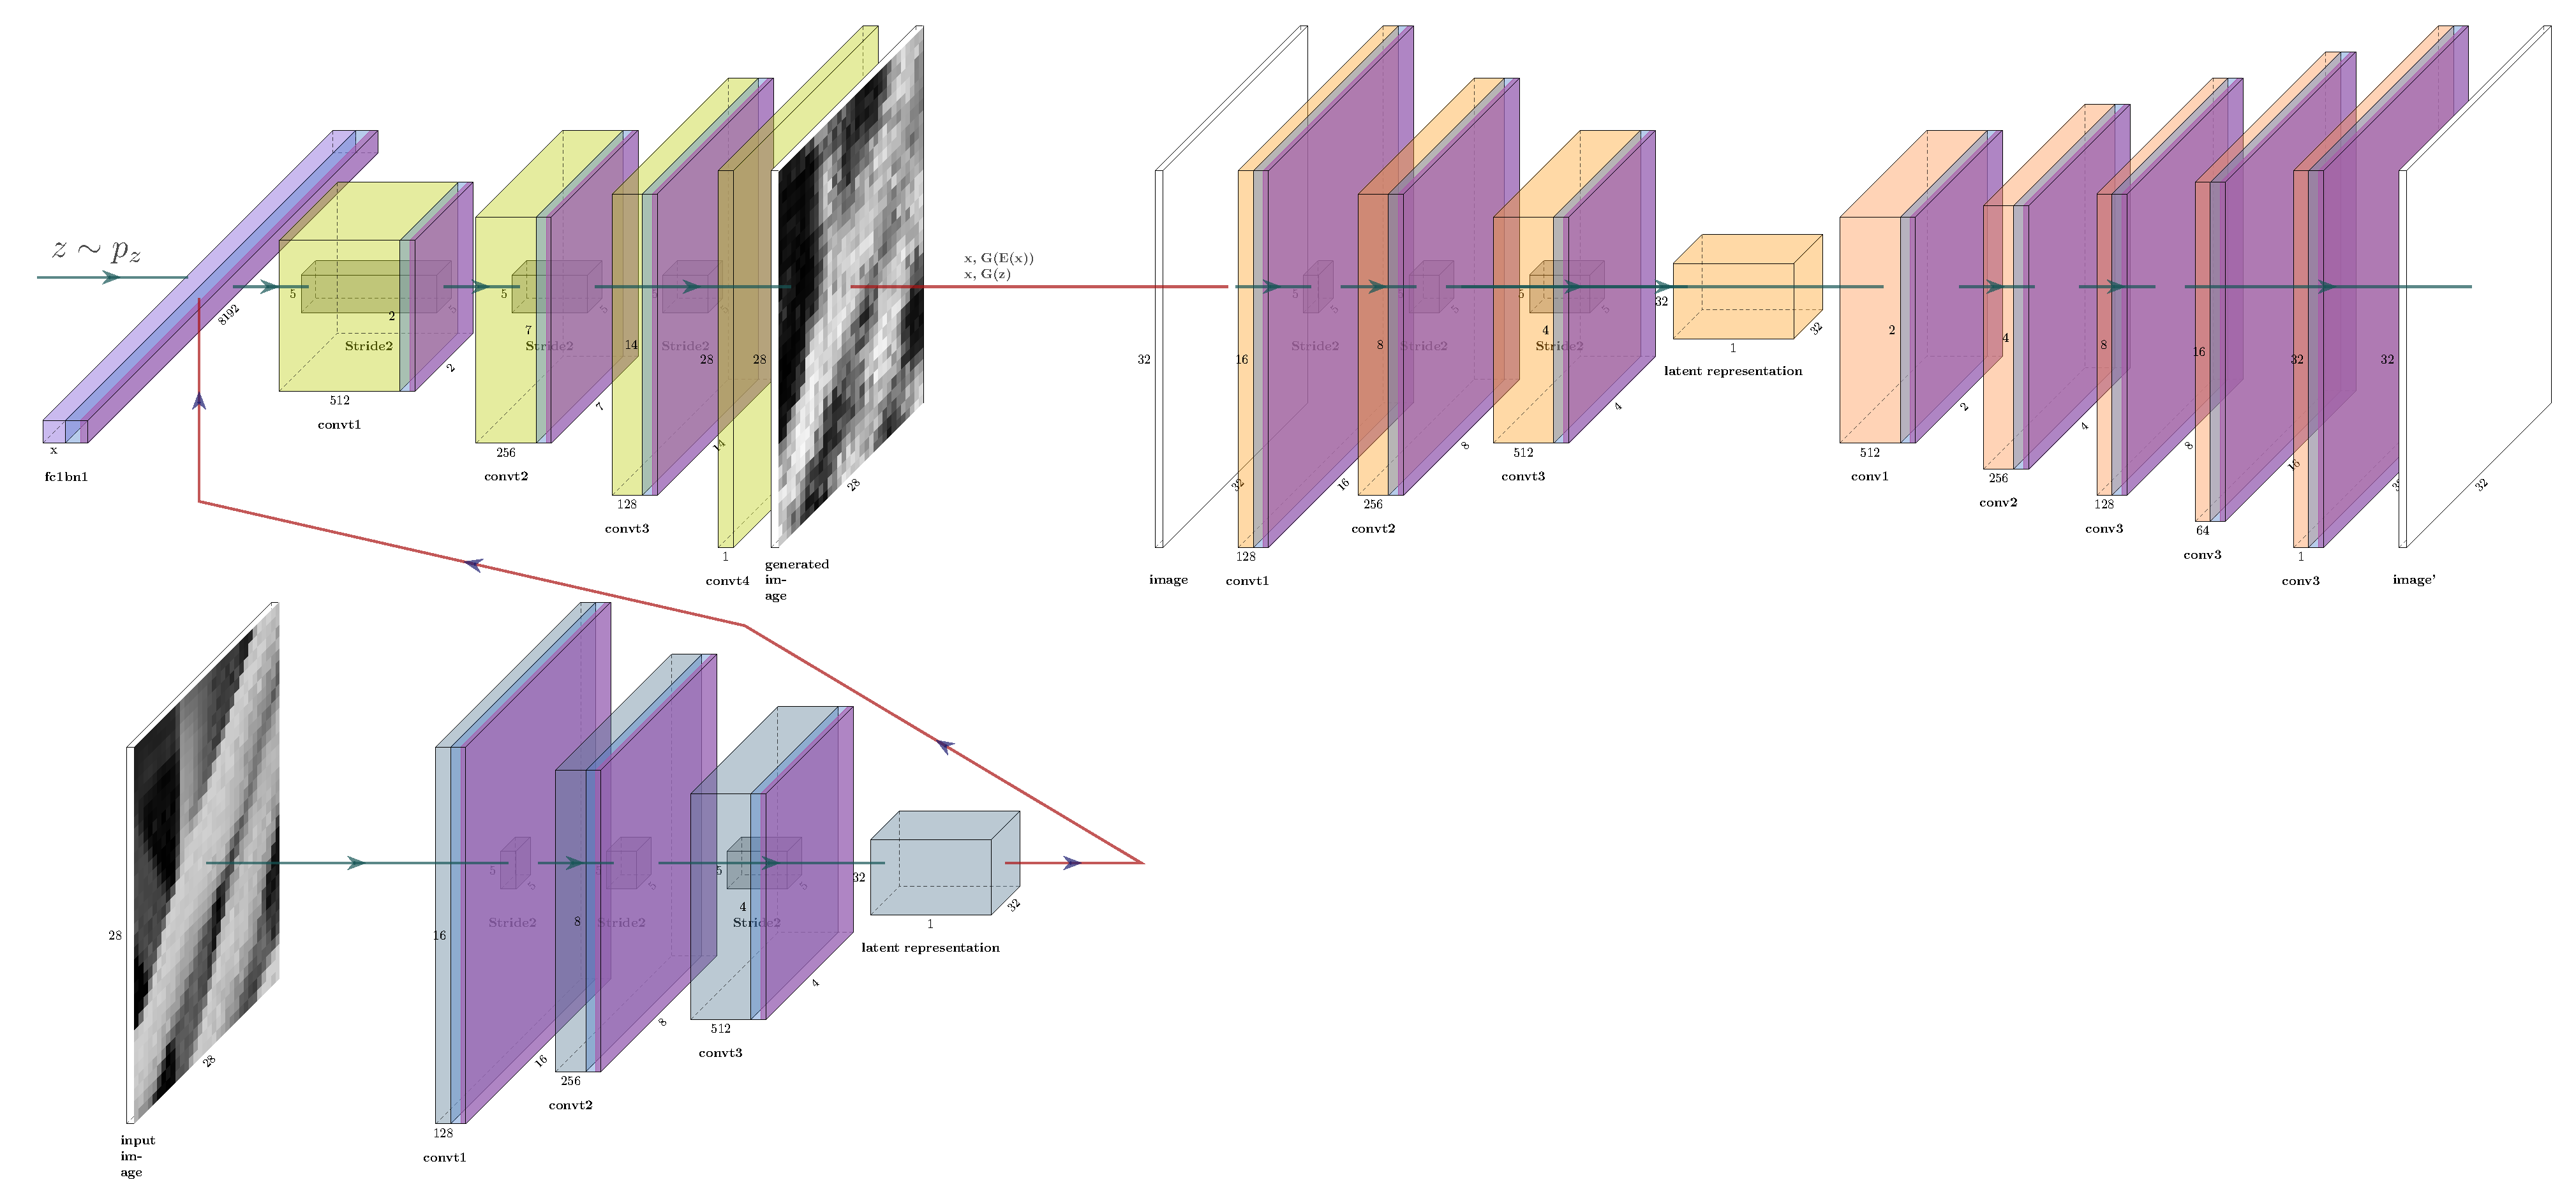
\includegraphics[width=1.0\textwidth]{encebgan}
	\caption{ENCEBGAN Model Overview }
	\label{fig:encebgan_model}
\end{figure}

\subsection{Anomaly Score Computation}

\begin{figure}[h!]
	\centering
	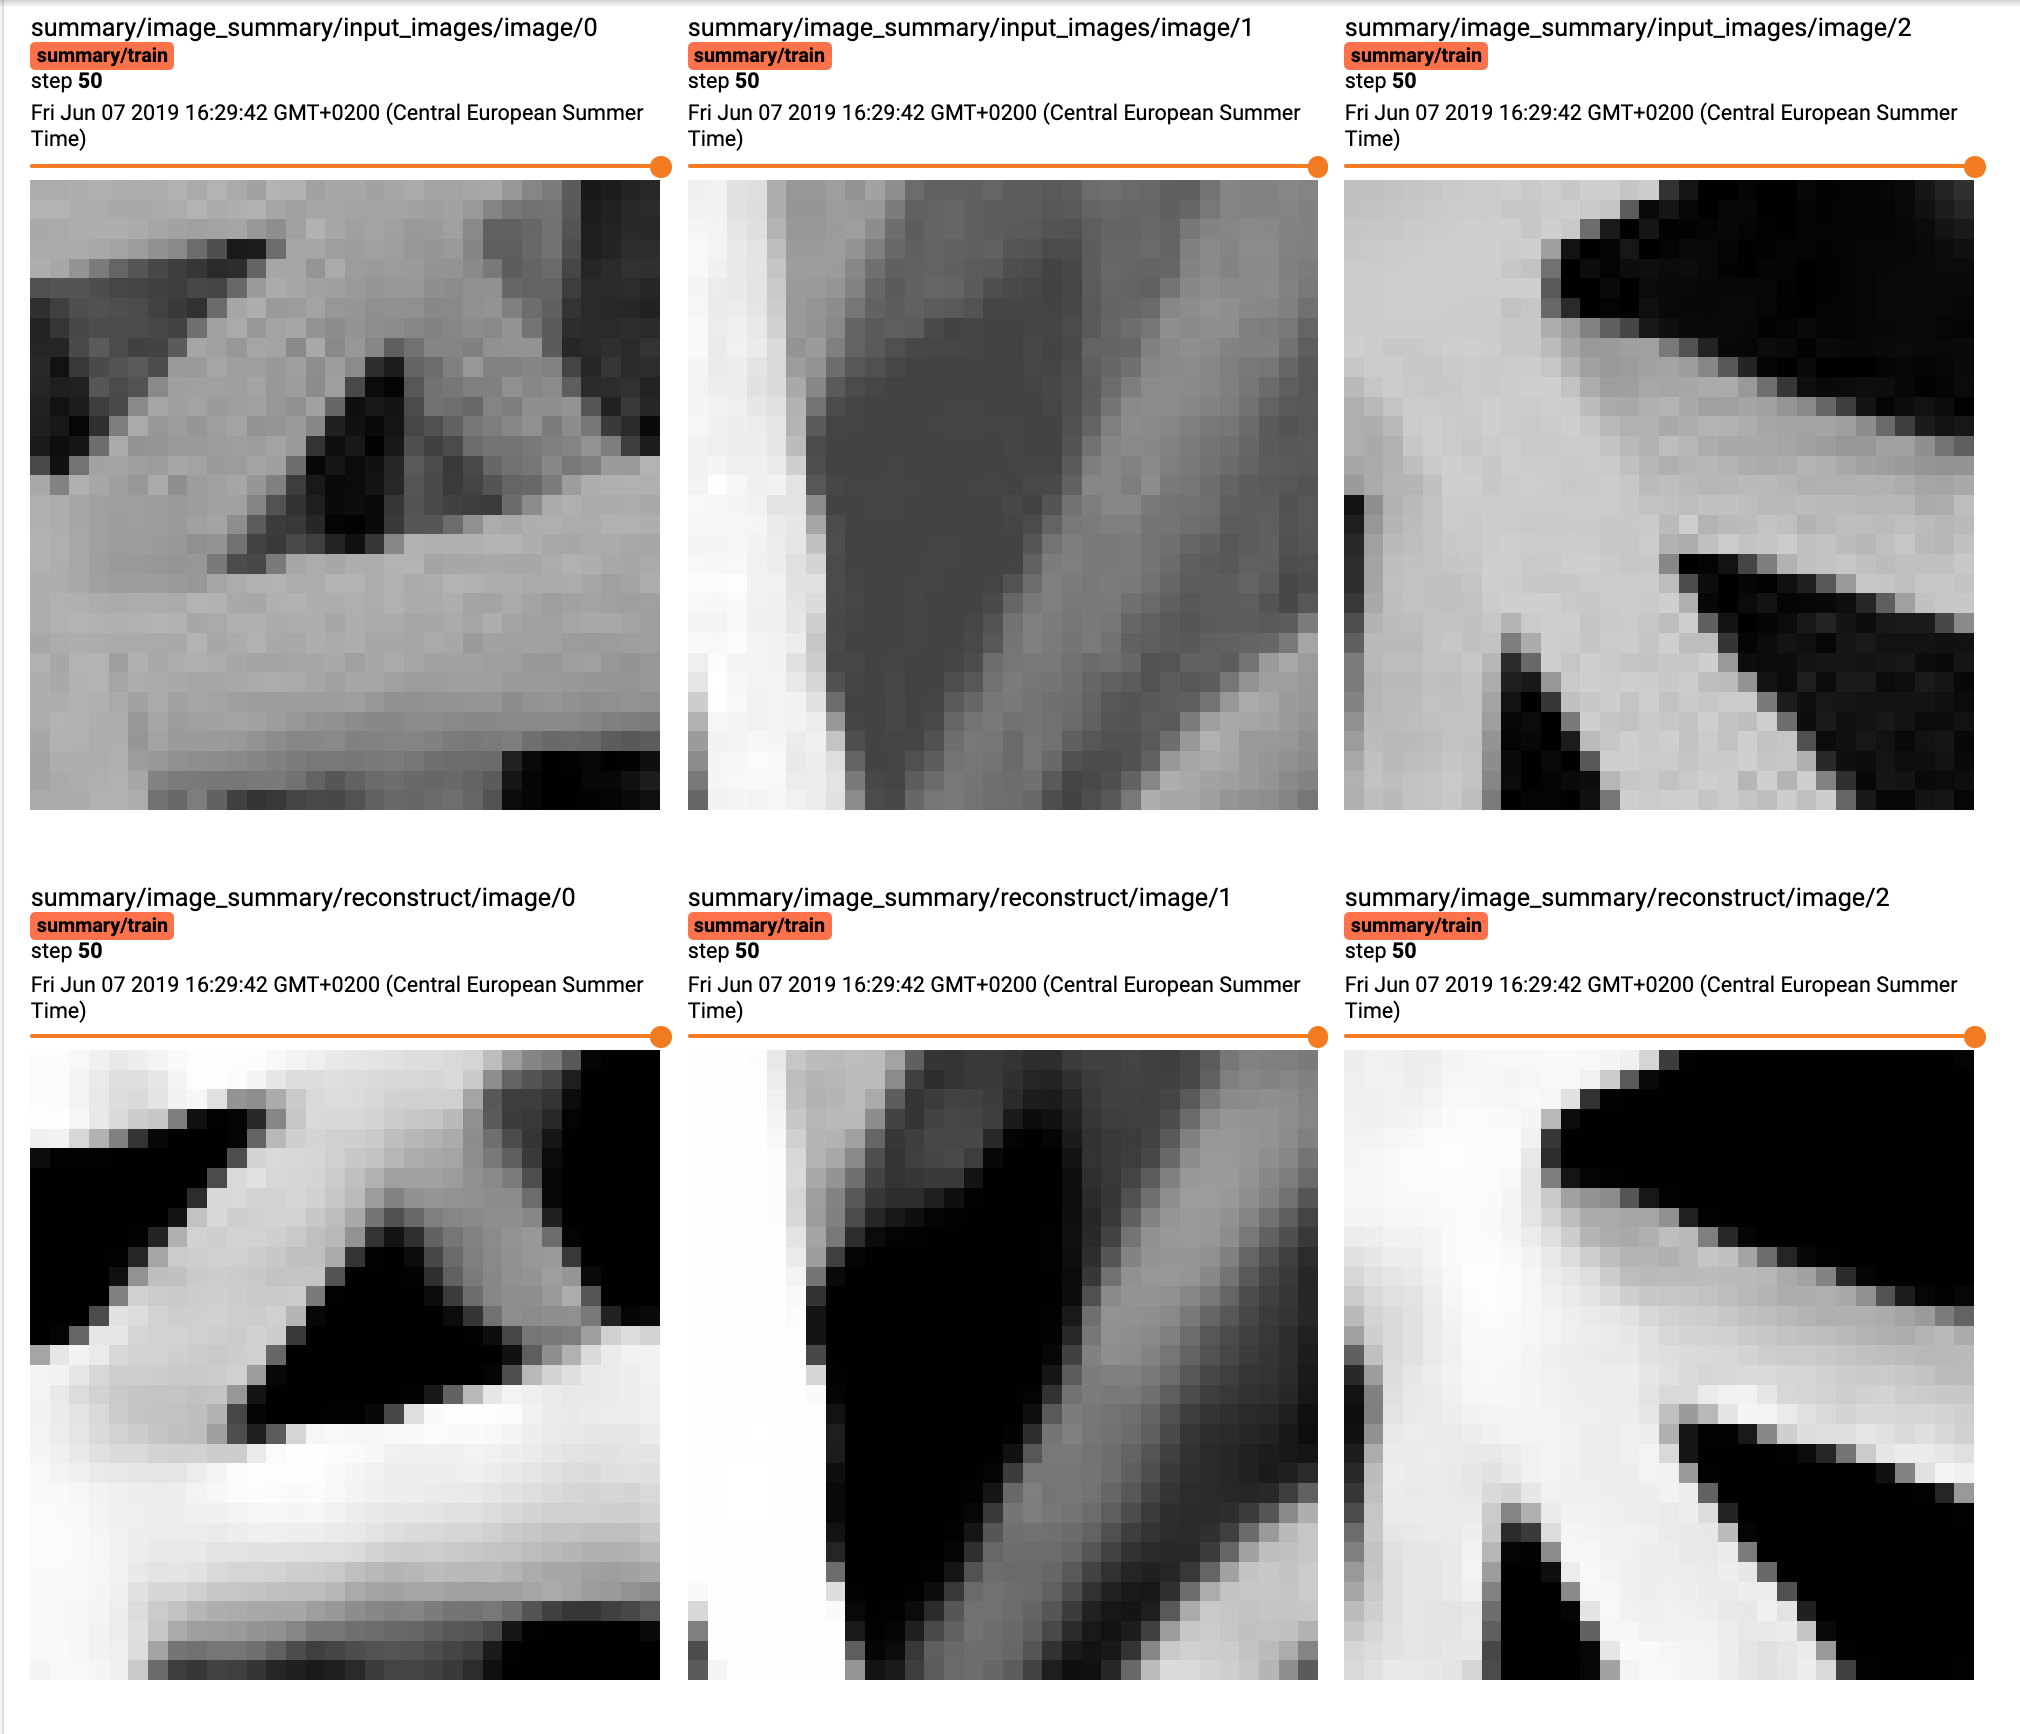
\includegraphics[width=0.75\textwidth]{reconstruct_ganomaly}
	\caption{SENCEBGAN Model Overview }
	\label{fig:sencebgan_model}
\end{figure}


\section{Sequentially Encoded Energy Based Generative Adversarial Network}
\label{sec:sencebgan}

\begin{figure}[h!]
	\centering
	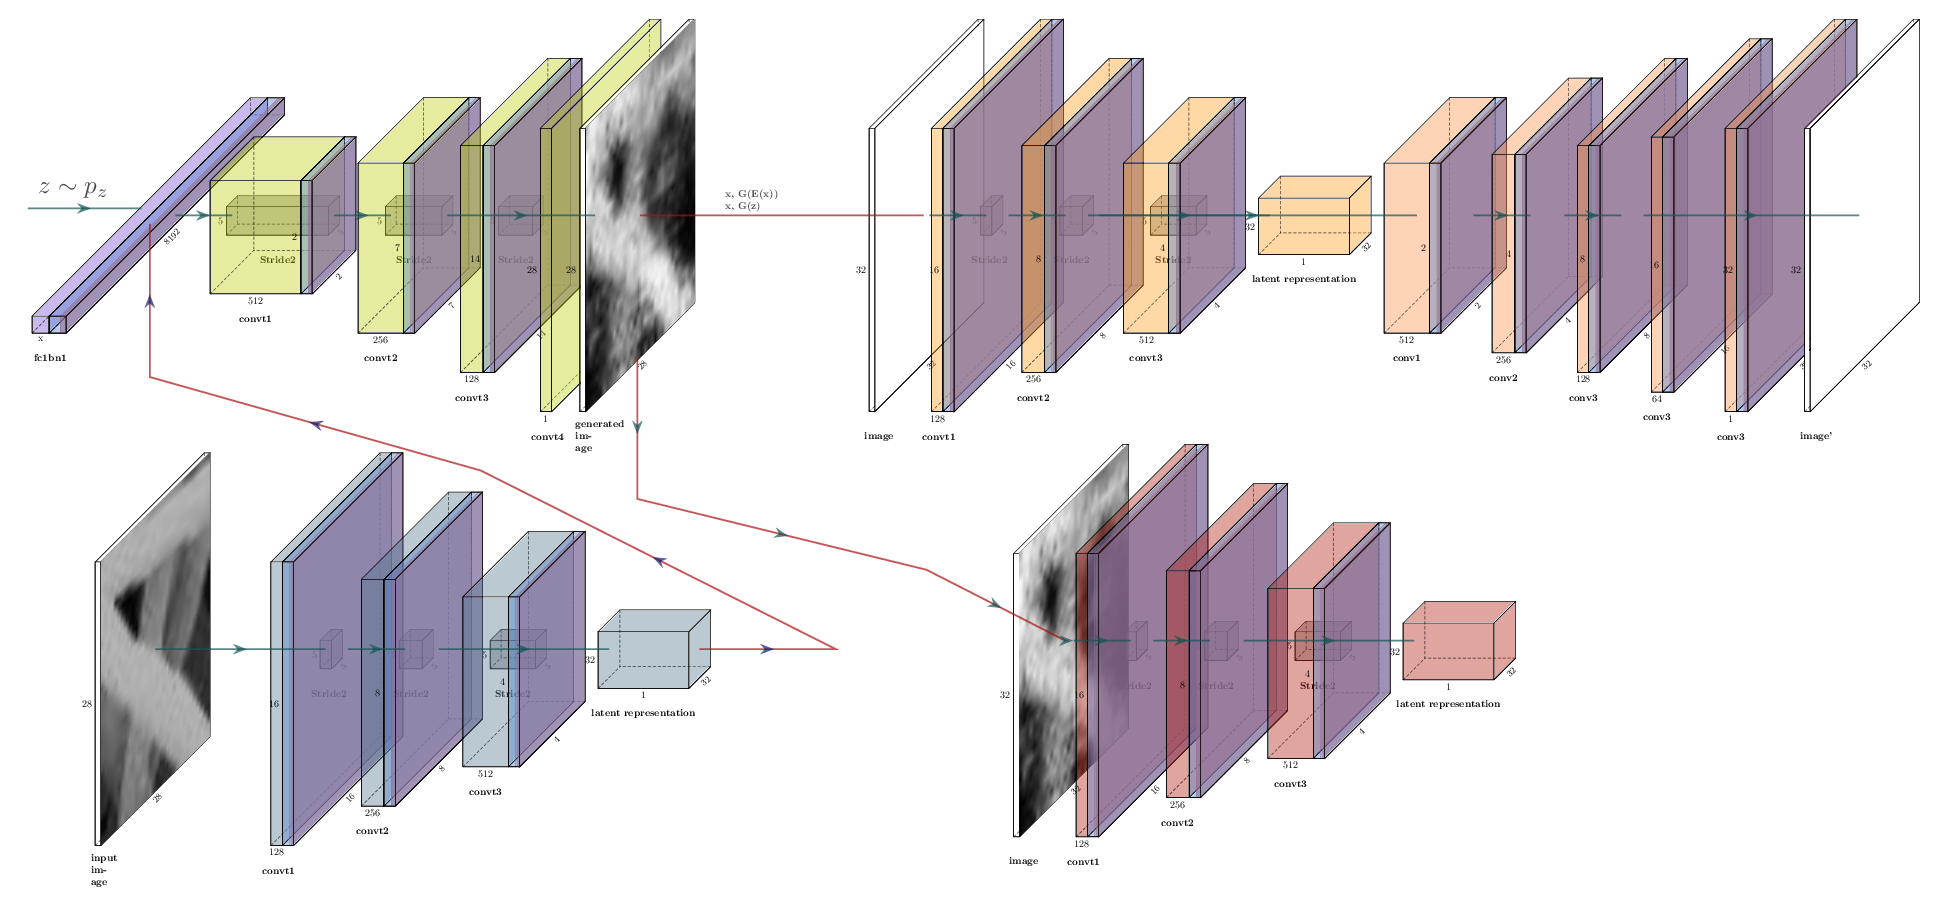
\includegraphics[width=1.0\textwidth]{sencebgan}
	\caption{SENCEBGAN Model Overview }
	\label{fig:sencebgan_model}
\end{figure}

\begin{figure}[h!]
	\centering
	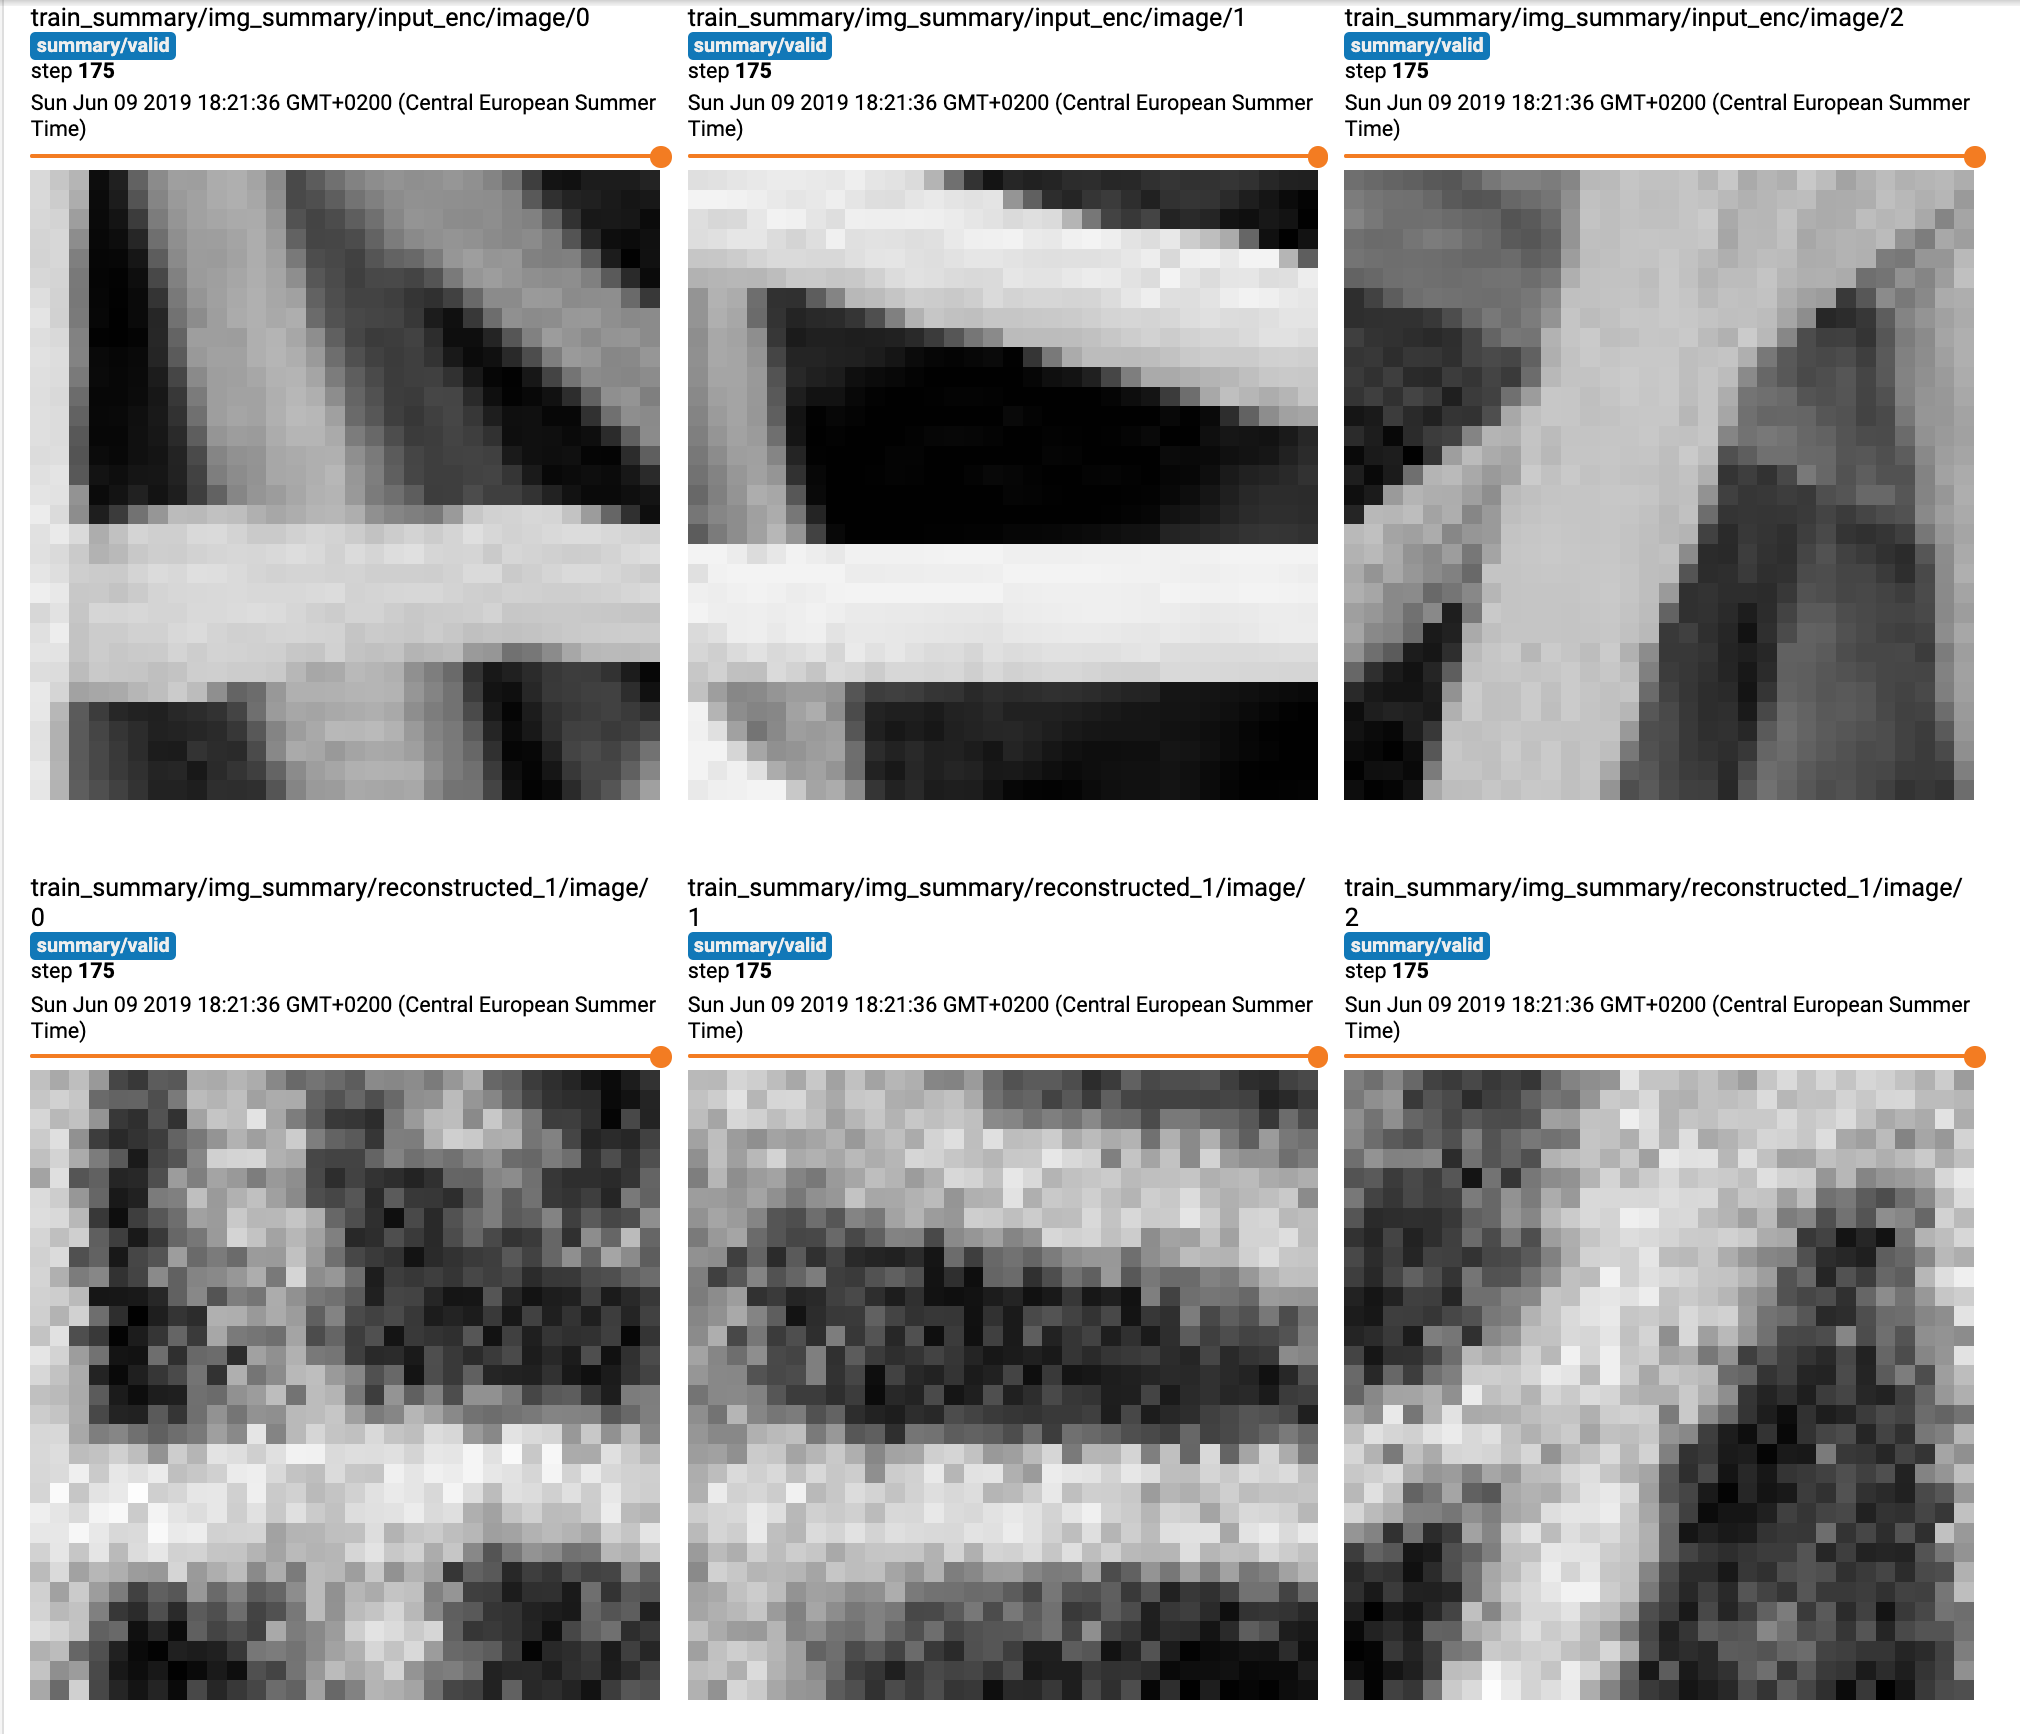
\includegraphics[width=0.75\textwidth]{reconstruct_sencebgan}
	\caption{SENCEBGAN Image Reconstruction  }
	\label{fig:sencebgan_model}
\end{figure}



\endgroup